% preamble

\documentclass[10pt]{article}
\usepackage[paperwidth=40in, paperheight=40in]{geometry}
\usepackage[usenames]{color} %used for font color
\usepackage{amssymb} %maths
\usepackage{amsmath} %maths
\usepackage[utf8]{inputenc} %useful to type directly diacritic characters

%%% Sans serif text font
\usepackage[scaled]{helvet}
\renewcommand*\familydefault{\sfdefault}\usepackage[T1]{fontenc}
%%%

\usepackage{skull}
\usepackage{tikz}
\usetikzlibrary{positioning}
\usetikzlibrary{arrows}
\usetikzlibrary{fit}
\usetikzlibrary{calc}
\usetikzlibrary{automata}
\usetikzlibrary{decorations.markings}
\usetikzlibrary{decorations.pathreplacing}

\tikzset{>=latex}
\tikzstyle{snode}=[black,draw=black,line width=1.5pt,shape=circle,fill=white,minimum size=8mm]
\tikzstyle{obnode}=[black,draw=black,line width=1.5pt,shape=circle,fill=black!20!white,minimum size=8mm]
\tikzstyle{detnode}=[black,draw=black,line width=1.5pt,densely dotted,shape=circle,fill=white,minimum size=8mm]
\tikzstyle{constnode}=[black,draw=black,line width=1.5pt,shape=rectangle,fill=white,minimum size=8mm]
\tikzstyle{mincnode}=[black,draw=black,line width=0.75pt,shape=rectangle,fill=white,minimum size=3mm]
\tikzstyle{blnode}=[white,draw=black,line width=1pt,shape=circle,fill=black,minimum size=1mm,font=\scriptsize,inner sep=1pt]
\tikzstyle{ylnode}=[black,draw=black,line width=1pt,shape=circle,fill=yellow,minimum size=1mm,font=\scriptsize,inner sep=1pt]
\tikzstyle{taro}=[->,line width=2pt,color=black]
\tikzstyle{thintaro}=[->,line width=0.75pt,color=black]
\tikzstyle{dtaro}=[->,line width=2pt, densely dotted,color=black]
\tikzstyle{smod}=[black, draw=black, line width=2pt, fill=white, shape=rectangle, rounded corners, minimum size=10mm, minimum width=20mm]
\tikzstyle{obmod}=[black, draw=black, line width=2pt, fill=black!20!white, shape=rectangle, rounded corners, minimum size=10mm, minimum width=20mm, minimum width=20mm]

\definecolor{shc}{RGB}{238,224,229}
\definecolor{shc2}{RGB}{182,152,195}
\definecolor{brnt}{RGB}{221,132,13}
\definecolor{sage}{rgb}{0.64, 0.76, 0.68}


\begin{document}
\[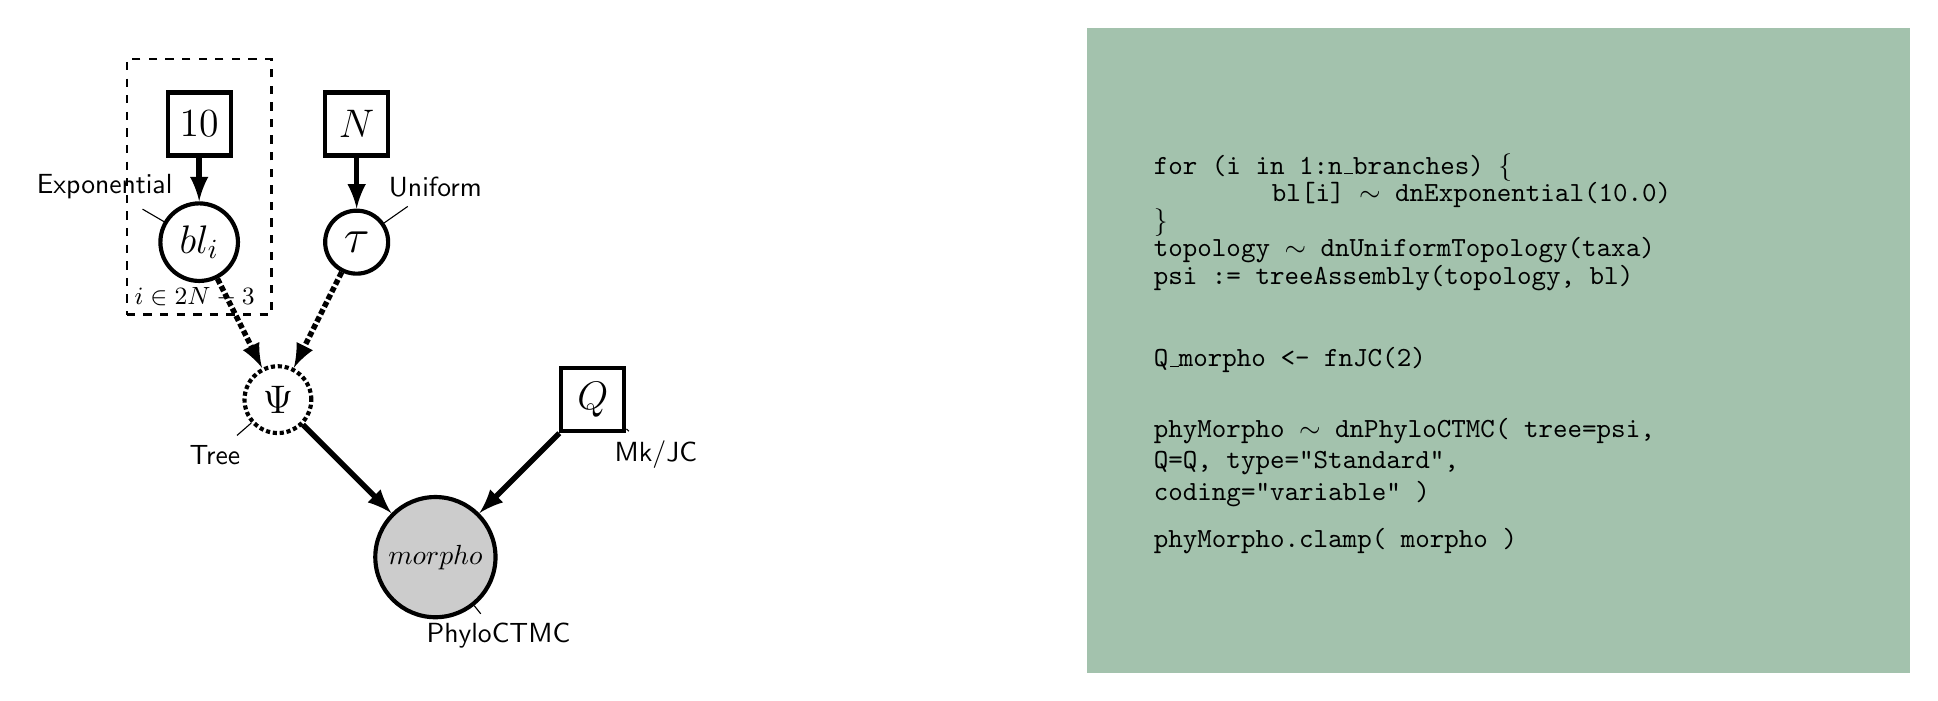
\begin{tikzpicture}
\node[obnode] (x) at (-5,1) {$morpho$};
\node (x_dist) at ($(x)+(0.8,-1.0)$) {PhyloCTMC};
\draw (x) -- (x_dist) ;
\node[constnode] (Q) at ($(x)+(2,2)$) {\Large $Q$};
\node (Q_dist) at ($(Q)+(0.8,-0.7)$) {Mk/JC};
\draw (Q) -- (Q_dist) ;
\node[detnode] (psi) at ($(x)+(-2,2)$) {\Large $\Psi$};
\node (psi_dist) at ($(psi)+(-0.8,-0.7)$) {Tree};
\draw (psi) -- (psi_dist);
\node[snode] (bl) at ($(psi)+(-1.0,2.0)$) {\Large $bl_i$};
\node[snode] (tau) at ($(psi)+(1,2.0)$) {\LARGE $\tau$};
\node (bl_dist) at ($(bl)+(-1.2,0.7)$) {Exponential};
\node (tau_dist) at ($(tau)+(1.0,0.7)$) {Uniform};
\draw (bl) -- (bl_dist);
\draw (tau) -- (tau_dist);
\node[constnode] (rate_bl) at ($(bl)+(0,1.5)$) {\Large $10$};
\node[constnode] (N) at ($(tau)+(0,1.5)$) {\Large $N$};
\node[rectangle,dashed, thick, inner sep=4mm, draw=black!100, fit = (rate_bl) (bl)] (bl_plate) {};
\node[anchor=south west,inner sep=3pt] at (bl_plate.south west) {\small $i \in 2N-3$};
\draw [taro] (rate_bl) -- (bl);
\draw [taro] (N) -- (tau);
\draw [dtaro] (tau) -- (psi);
\draw [dtaro] (bl) -- (psi);
\draw [taro] (Q) -- (x);
\draw [taro] (psi) -- (x);
\node (a1) at (4,0.25) { };
\node (a2) at (4,7.0) { };
\node (a3) at (13.0,2.75) { };
\node[rectangle, very thick, inner sep=6mm, fill=sage, fit = (a1) (a2) (a3)] (console) {};
\node (l1) at (4,5.95) [right]{\tt for (i in 1:n\_branches) \{};
\node (l1) at (5.5,5.6) [right]{\tt bl[i] $\sim$ dnExponential(10.0)};
\node (l1) at (4,5.25) [right]{\tt \}};
\node (l1) at (4,4.9) [right]{\tt topology $\sim$ dnUniformTopology(taxa)};
\node (l2) at (4,4.55) [right]{\tt psi := treeAssembly(topology, bl)};
\node (l8) at (4,3.5) [right]{\tt Q\_morpho <- fnJC(2) };
\node (l9) at (4,2.6) [right]{\tt phyMorpho $\sim$ dnPhyloCTMC( tree=psi, };
\node (l9) at (4,2.2) [right]{\tt  Q=Q, type="Standard",};
\node (l10) at (4,1.8) [right]{\tt coding="variable" ) };
\node (l10) at (4,1.2) [right]{\tt phyMorpho.clamp( morpho ) };
\end{tikzpicture}
\]
\end{document}